

\documentclass[main.tex]{subfiles}

\begin{document}

\chapter{Softening and fracture}
\label{LEC:SofteningFracture}

\paragraph{Outline}
We now include energy as a measure of stored and lost energy within a system into play. We also notice that if the material damage localizes due to softening behavior we observe an energy dissipation in a small volume of material while the whole domain/structure remains elastic. This observation brings to the idea to characterize the deterioration process of the structure by the means of energy release rate.

\paragraph{Addressed questions}
\begin{itemize}
    \item What is the consequence of the softening material behavior on the damage distribution within a structure?
    \item How can we numerically express the fact that the stress state in the localization zone remains unchanged during its "travel" through the structure?
    \item How to evaluate the stored and released energy from the load-displacement diagram of a test? 
\end{itemize}

\section{Is energy dissipation an objective material property?}

\mnote{Material model as a material point with memory}
Up to now, we have described the inelastic material behavior from the perspective of a material point
representing a small volume of a continuum.
In fact, we considered only a one-dimensional continuum represented by the interface between the two material components. We focused on a point on this interface and followed the stress and strain evolution at this point. 
The strain at the point was represented by the slip $s$ and the stress by the bond stress flow $\tau$.
Our goal was to describe the relation between 
\[
\tau(s; \boldsymbol{\theta}),
\]
i.e. between shear stress $\tau$, slip $s$  and state variables $\boldsymbol{\tau}$.
With state variables $\boldsymbol{\theta}$, exemplified by damage, plastic slip, kinematic or isotropic hardening, 
we introduced a kind of material point \textit{memory}.
Recall that in case of an explicitly prescribed \textit{memoryless} bond-slip law 
\[
\tau(s),
\]
as it was introduced in Chapter~\ref{LEC:BondBehavior}
there was no material memory and no path dependency. 
For more complex types of material behavior, exemplified by plasticity or damage, 
the memory in form of state variables has  been introduced to allow for  complex loading scenarios with unloading and reloading.

\mnote{Softening, stress concentration, discontinuity}
In this chapter we focus on the material behavior exhibiting softening. 
This means that the bond slip relation contains a descending branch as was the case e.g. in Example~\ref{e33_cfrp_and_concrete}. 
Such type of material behavior leads to a stress concentration within 
a small volume of material. This volume is called a process zone. 
In case of debonding, we can observe a propagation of the process zone 
throughout the embedded length for to increasing load. The debonding with a distinguished, propagating process zone can be observed in the Example~\ref{ex52_pullout_damage}
simulating the pullout behavior of a CFRP sheets from the concrete matrix using a damage-based softening model  Behind the process zone, 
a distinguished displacement discontinuity develops. Moreover, if the stress transfer across the newly emerged discontinuity is small, we can  regard it 
as a crack. In the pullout problem, this crack occurs in form of a slip line
that us usually referred to as a shear crack or mode II crack.

\mnote{Process zone}
In this case, the structural behavior can be directly related to the characteristics of the process zone. 
Then, the structural response can be described in an alternative way to the approaches described so far in chapters \ref{LEC:BondBehavior} and \ref{LEC:SofteningFracture}. Instead of regarding the local stress-strain response at every material point of the structure we can focus on the description of the small, inelastic process zone in an intermediate state of its propagation through the structure. Then, we calculate 
its impact on the surrounding structure where no inelastic effects occur. 
This can be done if the size of the process zone is small compared to the size of the structure. 

\mnote{Energy dissipation}
The characterization of the process zone includes particularly its size and the energy dissipation associated with its propagation through the structure.
Instead of defining the material behavior in terms of the stress-strain relation, we postulate that the size of the process zone and rate of energy dissipated within it remains constant during its propagation through the structure. Thus, we regard it as a material property associated with particular material, objectively characterizing its localization process of damage into a material discontinuity, i.e. crack. As already emphasized, this kind of
description is only possible for materials exhibiting strain-softening that are denoted as brittle or quasi-brittle. Examples of such materials 
include concrete, fiber-reinforced concrete and ceramics.

\mnote{Introductory example}
We will start the explanation by revisiting the example of the pullout test with a damage function that introduces softening. 
In particular, we will describe the debonding of FRP sheet from the concrete matrix observed in the test and evaluate the amount of work supplied to the structure by the imposed loading.

\mnote{Correspondence between fracture and damage}
Our goal is to prepare the platform for the general explanation of the correspondence between the theoretical concepts of fracture mechanics, i.e. the energetic characterization of the material disintegration, and between the strain-softening types of models used in the finite element simulation of brittle materials exhibiting cracking.

\textsave{
\mnote{Types of load control}
In the course of the chapters \ref{LEC:CohesiveZone} and \ref{LEC:CrackPropagation} we have encountevred three different ways how to control the nonlinear simulation of a test exhibiting strain-localization and, eventually, snap-back. Within the topic 6.3 showing the cohesive crack model, we have controlled the calculation by linearly increasing the crack opening. In topic 7.1 we controlled the response of a bar by decreasing stress level. In topic 7.3, the displacement control has been used. It is useful to realize that all these possibilities can be realized in designing experimental setups. However, most of the experiments are conducted using the displacement control.
}

\section{Energetic interpretation of the nonlinear structural response}

\begin{figure}[h!]
	\centering
  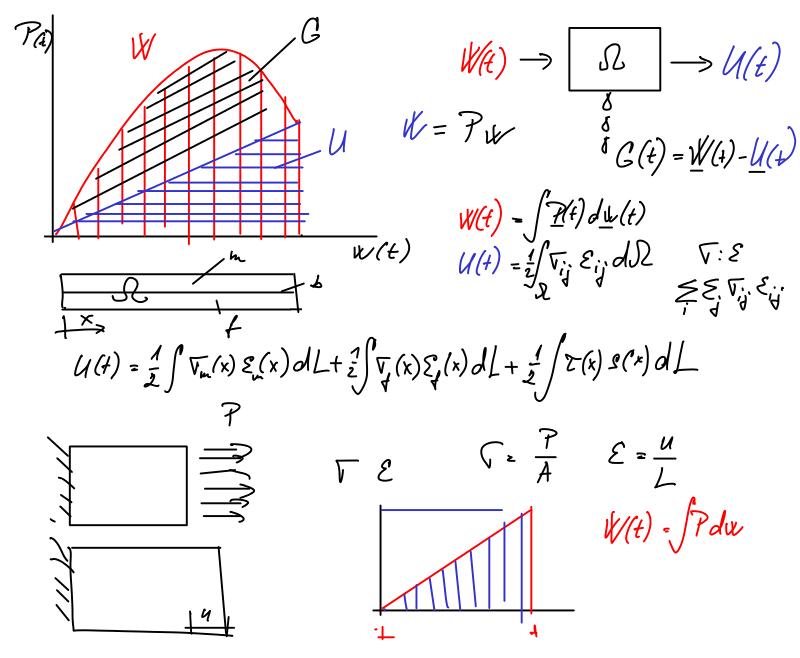
\includegraphics[width=1.0\textwidth]{drawings/energy_dissipation.png}
	\caption{Energy bilance for the pullout with constant bond-slip law}
	\label{FIGDrawingEnergyPullout}
\end{figure}

\textsave{
\begin{figure}[!h]
	\centering
  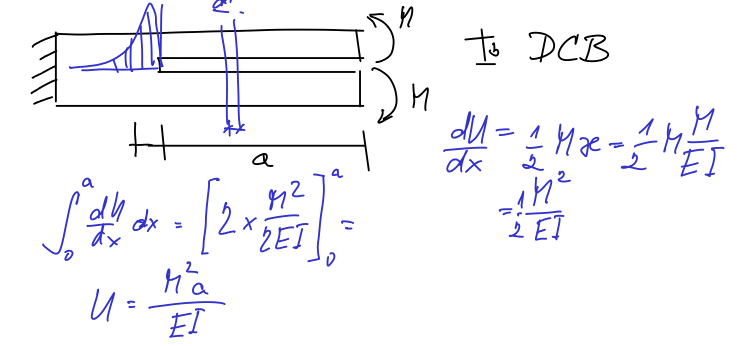
\includegraphics[width=1.0\textwidth]{drawings/double_cantilever_beam.png}
	\caption{Evaluation of supplied and stored energy in a double cantilever beam}
	\label{FIGDrawingDCB}
\end{figure}
}

\section{General formula for energy supply}

\mnote{Work of external force}
Assume a tensile specimen with the total energy supply given as an integral of the load  over the displacement variable  $u$
\begin{align}
\label{eq:work_supply}
W = \int P(u) \; \mathrm{d}u
\end{align}
Assuming linear elastic material behavior we can employ the equilibrium condition and kinematic relation to link the load  directly to the control displacement $u$ as
\begin{align}
P = A \sigma = A E \varepsilon = A E \frac{1}{L} u,
\end{align}
where $E$ denotes the Young’s modulus, $\sigma$ the stresses, $A$ the cross-sectional area and $\varepsilon$ the strain. Then the total energy supply reads
\begin{align}
\label{eq:elastic_energy_supply}
W = 
\frac{1}{L} A E \int u \; \mathrm{d}u
=
\frac{1}{2L} A E u^2
=
\frac{1}{2} P u
\end{align}
The stored energy is \mnote{Stored elastic energy}
represented by the area below the unloading branch integrated over the whole volume of the structure.
In case of the tensile specimen with uniform profile of stress and strain, the integral reduces to
\begin{align}
\mathcal{U}
=
\frac{1}{2}
\int_\Omega
\sigma
\varepsilon
\;
\mathrm{d}x
=
\frac{1}{2}
A L \sigma \varepsilon
=
\frac{1}{2}
P u
\end{align}
By evaluating the difference between supplied and stored energy, we obtain the obvious result
\begin{align}
G = W - \mathcal{U} = 0
\end{align}
rephrasing the fact that the supplied energy is stored in the specimen without any loss.

In case of a pullout test, the work supply remains unchanged. It can be evaluated using Eq.~\ref{eq:work_supply}.
The stress distribution is not uniform anymore so that we need to evaluate the integral explicitly.
In cases considered so far we assumed linear elastic behavior of the matrix and of the reinforcement.
Thus, the integral over the volume of the specimen can be decomposed into
\begin{align}
    \label{eq:stored_energy_pullout}
\mathcal{U}
=
\frac{1}{2}
\int_{\Omega_\mathrm{m}}
\sigma_\mathrm{m}(x)
\varepsilon^\mathrm{el}_\mathrm{m}(x)
\;
\mathrm{d}x
+
\frac{1}{2}
\int_{\Omega_\mathrm{f}}
\sigma^\mathrm{el}_\mathrm{f}(x)
\varepsilon_\mathrm{f}(x)
\;
\mathrm{d}x
+
\frac{1}{2}
\int_{\Omega_\mathrm{mf}}
\tau_\mathrm{mf}(x)
s^\mathrm{el}_\mathrm{mf}(x)
\;
\mathrm{d}x
\end{align}

This equation is valid for any kind of material behavior in the bond zone (damage or plasticity), (softening or hardenign). 
Its evaluation may be regarded as counting of intact, undamaged material links/spring in every single
material point along the bond zone. The elastic springs of the matrix remain undamaged by assumption. The bond between
the material components may release energy depending on the material behavior that we assume.
However, if we can solve the boundary value problem numerically as we did in the previous 
Chapters assuming damage or plasticity of the bond interface, we can use Eq.~\ref{eq:stored_energy_pullout}
to evaluate the stored energy and, thus, the overall energy dissipation in the pullout problem.


To explain the concept in simple terms, let us return back to the example of the analytically solved
pullout problem given Chapter \ref{LEC:PullOut} with the interface governed by a constant, frictional behavior:


\textsave{
The displacement along the embedded length was obtained as
\label{eq:displacement_5}. Its derivative along the $x$ coordinate delivers the strain $\varepsilon$ as
\begin{align}
\label{eq_eps_f_pullout_rigid}
\varepsilon = \frac{P}{E_\mathrm{f}A_\mathrm{f}} + \frac{p\tau x}{A_\mathrm{f}E_\mathrm{f}}
\end{align}
}

\begin{bmcsex}{Energy dissipation in a pullout test with constant bond}{eq_61_energy_dissipation}
The analytical formula of work supply, stored energy and energy dissipation
has been derived in Sec.~\ref{LEC:PullOut} for a rigid matrix and constant level of bond stress.
Using the analytical solution we have all state variable needed to evaluate the stored energy available. 

\paragraph{Task:} Consider the pullout state with a fixed value $w$

\paragraph{Question:} What the is amount of energy stored in the pullout specimen at a given control pullout displacement:
\begin{itemize}
    \item assuming that the bar has infinite stiffness
    \item assuming that the bar has a finite  stiffness $E$ and area $A$?
\end{itemize}

\paragraph{Question:} Which amount of energy dissipated in the state $w$ is larger?  
\begin{itemize}
    \item the one with a bar of infinite stiffness? 
    \item the one with bar of an finite stiffness $A$?
\end{itemize}
Use the example notebook to confirm your answers to the the questions.
\end{bmcsex}

\end{document}